\subsection{Classical Algebraic Multigrid (AMG)}

\definition{Classical Algebraic Multigrid (AMG)} is a numerical \textbf{method for solving large systems of equations}, especially those arising from the \textbf{discretization of partial differential equations}.

\highspace
It is a \textbf{type of multigrid method that uses matrix coefficients to construct a hierarchy of grids} rather than relying on geometric information (such as the V-cycle scheme). It aims to speed up the convergence of iterative methods by combining smoothing operations with coarse grid corrections.

\highspace
\begin{flushleft}
    \textcolor{Green3}{\faIcon{check-circle} \textbf{Why is AMG one of the best MG methods?}}
\end{flushleft}
When we think about how the V-cycle works, we notice an interesting thing. Each MG tool presented in the previous pages requires an interpretation of the geometric properties of the problems. Unfortunately, especially in the real world, it is very difficult to understand the geometric relationship, and mainly it avoids the coding necessary for a true multigrid implementation (we mean an implementation of "how can we geometrically pass from a fine to a coarse grid without losing important details or conditions?).

\highspace
The \textbf{main goal of the AMG method is its \emph{geometric independence}}. Unlike geometric multigrid methods, which rely on the geometric structure of the problem (grid spacing, shape, etc.), AMG \textbf{constructs its grid hierarchies based purely on the algebraic structure of the system matrix}. This makes it highly versatile and applicable to a wide range of problems, including those with complex geometries or unstructured grids. This is one of the most important differences, but the AMG also has other good points (efficiency, applicability, etc.).

\highspace
\begin{flushleft}
    \textcolor{Green3}{\faIcon{tools} \textbf{AMG Basis}}
\end{flushleft}
The method is divided into several theoretical concepts:
\begin{enumerate}
    \item Algebraic Multigrid (AMG) makes extensive use of \textbf{\underline{graph-based}} concepts. The \textbf{system matrix} (representing the discretized problem) can be viewed as a \textbf{graph}. Each \textbf{node in the graph corresponds to a grid point}, and each \textbf{edge represents a connection} (or interaction) \textbf{between grid points}. For example, the following sparse matrix has the corresponding graph.
    \begin{equation*}
        A = \begin{bmatrix}
            * & * & * & * & * & * \\
            * & * & * & 0 & 0 & 0 \\
            * & * & * & * & * & 0 \\
            * & 0 & * & * & * & 0 \\
            * & 0 & * & * & * & 0 \\
            * & 0 & 0 & 0 & 0 & *
        \end{bmatrix}
    \end{equation*}
    
    \begin{center}
        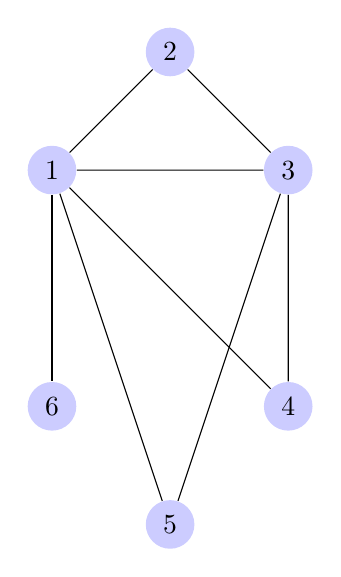
\begin{tikzpicture}[scale=1.5, every node/.style={circle, fill=blue!20}]
            \node (1) at (0, 2) {1};
            \node (2) at (1, 3) {2};
            \node (3) at (2, 2) {3};
            \node (4) at (2, 0) {4};
            \node (5) at (1, -1) {5};
            \node (6) at (0, 0) {6};
    
            \draw (1) -- (2);
            \draw (1) -- (3);
            \draw (1) -- (4);
            \draw (1) -- (5);
            \draw (1) -- (6);
    
            \draw (2) -- (3);
    
            \draw (3) -- (4);
            \draw (3) -- (5);
        \end{tikzpicture}
    \end{center}


    \item Classical AMG is based on the observation that the \textbf{algebraic smooth error varies slowly in the direction of the matrix's relatively large (negative) coefficients}. This gives us an algebraic way to track smooth errors. However, we still need to define large.

    \begin{definitionbox}[: strong connection]
        Given a threshold $\theta \in \left(0, 1\right)$ we say that $i$ is \textbf{strongly connected} with $j$ if:
        \begin{equation}
            -a_{i,j} \ge \theta \underset{k \ne i}{\max}\left(-a_{i,k}\right)
        \end{equation}
        Let us denote by $S_{i}$ the set of vertices that $i$ is strongly connected to by:
        \begin{equation}
            S_{i} = \left\{j \in N_{i} \: : \: i \text{ strongly connects to } j\right\}
        \end{equation}
        Where:
        \begin{equation*}
            N_{i} = \left\{j \ne i \: : \: a_{i,j} \ne 0\right\}
        \end{equation*}
    \end{definitionbox}
    
    \noindent
    This gives us a strength matrix $S$, with $S_{i}$ as its $i$-th row. AMG uses the concept of \emph{strong connection} to \textbf{decide how strongly nodes (grid points) are connected}. This is based on the matrix coefficients. Strong connections are those \textbf{where the matrix coefficients are relatively large}, indicating significant interactions between grid points.


    \item \textbf{\underline{Standard Coarsening}}. Standard coarsening in AMG involves \textbf{reducing the number of variables} (or degrees of freedom) \textbf{in the problem}. This is achieved by \textbf{selecting a subset of nodes}, known as coarse nodes (\textbf{C-vertices}), while the \textbf{remaining nodes become} fine nodes (\textbf{F-vertices}). The \textbf{goal is to simplify the problem while preserving its essential characteristics}.
    
    \begin{itemize}
    	\item \textbf{C-vertices} (Coarse nodes): These are the selected nodes that will form the coarse grid.
    	
    	\item \textbf{F-vertices} (Fine nodes): These are the remaining nodes that are not selected as coarse nodes.
    \end{itemize}
    To put it simply, in AMG we deal with the original problem on a \emph{fine grid}. However, solving large problems directly on this fine grid can be computationally expensive. To simplify, we \textbf{create several \dquotes{coarser} versions of this grid}, in which the \textbf{problem size is progressively reduced}. This process is called \emph{standard coarsening}.
    
    \begin{flushleft}
    	\textcolor{Green3}{\faIcon{question-circle} \textbf{How can we apply the Standard Coarsening?}}
    \end{flushleft}
    \textbf{\underline{It requires an observation before use}}. The oscillatory error should not be a problem, as this error is typically easier to reduce using standard relaxation methods on fine grids. However, the real dilemma is the smooth error, which can't be reduced by simple relaxation methods. \textbf{When applying standard coarsening, we need to focus on reducing smooth error while building each coarse grid group and preserving the most fundamental information}.
    
    \textbf{\underline{Implementation}}. To achieve this, we need to approach the problem from an algebraic point of view. The smooth error tends to vary slowly along strong connections (edges in the graph). Essentially, strong connections represent significant interactions or relationships between nodes (vertices). By \textbf{coarsening in the direction of} these \textbf{strong connections}, we \textbf{preserve the most critical aspects of the problem}, resulting in a more accurate and efficient MG method. In other words, we focus our coarsening efforts on the most \dquotes{meaningful} parts of the graph, where the important information is.
    
    \textbf{\underline{What happens in practice}}. In practice, standard coarsening \textbf{divides the vertices into} Coarse (\textbf{C-vertices}) and Fine (\textbf{F-vertices that are strongly connected to the C-vertices}) sets. The main idea is to \textbf{ensure that each F-vertex has a strong connection to at least one C-vertex}. This allows us to approximate the values at the F-vertices by a linear combination of the values at the C-vertices, preserving the important relationships in the original problem.
    
    \textbf{\underline{What happens after Standard Coarsening}}. The values at the F-vertices can be expressed as a weighted combination of the values at their neighboring C-vertices. This ensures that the coarser problem is a good approximation of the finer problem.
    
    \newpage
    
    \begin{flushleft}
    	\textcolor{Green3}{\faIcon{tools} \textbf{General Coarsening Algorithm}}
    \end{flushleft}
    Given a strength matrix $S$ indicating the strong connections between nodes, the algorithm is:
    \begin{enumerate}
    	\item \textbf{\underline{Initialization}}. We create an empty set $C$ for Coarse vertices and an empty set $F$ for Fine vertices.
    	
    	\item \textbf{\underline{Select an independent set of C-vertices}}. Choose an independent set of C-vertices from the graph of $S$. An independent set means that no two selected C-vertices are directly connected by a strong connection.
    	
    	The selection process is as follows:
    	\begin{enumerate}
    		\item \textbf{\underline{Choose a C-vertex}}. Start with a node and mark it as a C-vertex. In general, we start at the node with the highest number of strong connections (or highest weight, if applicable).
    		\item \textbf{\underline{Populate Fine vertices set}}. All vertices strongly connected to the previously selected C-vertex become F-vertices.
    		\item \textbf{\underline{Repeat}}. We repeat the process by selecting another vertex from the undecided vertices as a C-vertex and making the vertices strongly connected to it as F-vertices.
    		\item \textbf{\underline{Stop when all vertices are classified as either C-vertex}}\break \textbf{\underline{or F-vertex}}.
    	\end{enumerate}
    	
    	\item \textbf{\underline{Select additional C-vertices}}. Ensure that every F-vertex has a strong connection to at least one C-vertex. If any F-vertex is not strongly connected to a C-vertex, convert that F-vertex into a C-vertex to ensure the interpolation requirements are satisfied.
    \end{enumerate}
\end{enumerate}

\begin{flushleft}
	\textcolor{Red2}{\faIcon{bookmark} \textbf{Interpolation}}
\end{flushleft}
Interpolation is used to \textbf{estimate unknown values at fine nodes (F-nodes) using the known values at coarse nodes (C-nodes)}. It’s crucial for maintaining accuracy and efficiency.

Let $\mathbf{e} = \left( e_{1}, e_{2}, \dots, e_{i}, \dots \right)$ be the error; a simple characterization of algebraic smooth error is $A\mathbf{e} \approx 0$. In other words:
\begin{equation}
	a_{i,i} e_{i} + \displaystyle\sum_{j \in N_{i}} a_{i,j}e_{j} \approx 0 \hspace{2em} i \in F
\end{equation}
The idea is that we want to choose proper weight $w_{i,j}$ such that for any algebraic smooth errors:
\begin{equation*}
	e_{i} \approx \displaystyle\sum_{j \in C} w_{i,j}e_{j} \hspace{2em} i \in F
\end{equation*}
But if we define for $i \in F$:
\begin{itemize}
	\item $C_{i}$ the C-points strongly connected to $i$:
	\begin{equation*}
		C_{i} = C \cap N_{i}
	\end{equation*}
	
	\item $F_{i}^{S}$ the F-points strongly connected to $i$:
	\begin{equation*}
		F_{i} = F \cap N_{i}
	\end{equation*}
	
	\item $C_{i}^{S} = C \cap S_{i}$
	
	\item $N_{i}^{W}$ all points weakly connected to $i$:
	\begin{equation*}
		N_{i}^{W} = \dfrac{N_{i}}{\left(C_{i}^{S} \cup F_{i}^{S}\right)}
	\end{equation*}
\end{itemize}
We can rewrite the characterization of algebraic smooth error as:
\begin{equation}
	a_{i,i} e_{i} + \displaystyle\sum_{j \in N_{i}} a_{i,j}e_{j} = 0 \hspace{2em} \alpha = \dfrac{
		\displaystyle\sum_{j \in N_{i}} a_{i,j}
	}{
		\displaystyle\sum_{j \in C_{i}^{S}} a_{i,j}
	}
\end{equation}
We conclude that the \textbf{formula of direct interpolation} is:
\begin{equation}
	w_{i,j} = \alpha\dfrac{a_{i,j}}{a_{i,i}} \hspace{2em} i \in F, \: j \in C_{i}^{S} \hspace{2em} \alpha = \dfrac{
		\displaystyle\sum_{j \in N_{i}} a_{i,j}
	}{
		\displaystyle\sum_{j \in C_{i}^{S}} a_{i,j}
	}
\end{equation}
The above direct interpolation can be applied as long as $C_{i}^{S}$.

\highspace
\begin{flushleft}
	\textcolor{Red2}{\faIcon{dollar-sign} \textbf{How much does it cost?}}
\end{flushleft}
The cost of each iteration in the Algebraic Multigrid (AMG) method primarily \textbf{depends on the operations involved}, such as smoothing, restriction, interpolation, and correction (the all tools that we have already discussed in the previous pages!). The cost is \textbf{generally linearly proportional to the problem size}. This means that as the problem size increases, the cost increases linearly, making AMG methods efficient for large-scale problems.

\highspace
However, leaving aside the iteration cost for the moment, the \textbf{AMG method is the best of the multigrid methods because the construction of the MG hierarchy is done using only information from the matrix and not from the geometry of the problem}. This is the main and most important key. This is one of the most important reasons to choose AMG, especially in real practice problems.

\highspace
\begin{flushleft}
	\textcolor{Green3}{\faIcon{network-wired} \textbf{Can it be parallelized?}}
\end{flushleft}
AMG is not only the best because it is geometric independent, but also because it lends itself very well to parallelization! In general, \textbf{AMG methods are well suited for parallelization, especially for large problems}. The multi-level structure of AMG allows the workload to be distributed across multiple processors. However, the efficiency of parallelization depends on the specific implementation and the problem to be solved (of course). Optimizations and careful communication management can help achieve better parallel performance.
